\documentclass{article}
\usepackage{iclr2027_conference,times}

\input{math_commands.tex}

\usepackage[colorlinks=true,linkcolor=black!70!blue,citecolor=black!70!blue,urlcolor=black!70!blue]{hyperref}
\usepackage{url}
\usepackage{graphicx}
\usepackage{booktabs}
\usepackage{xcolor}
\usepackage{enumitem}
\usepackage{amsmath,amssymb,amsfonts,amsthm}
\usepackage{microtype}
\usepackage{multirow}
\usepackage{comment}   % appendix.tex hides draft notes in a comment environment

% Draft markers. Every marker names the evidence needed to remove it.
\definecolor{tbdcol}{HTML}{C0561B}
% TBD notes are shown by default.  To omit them all, either uncomment the
% \showtbdfalse line below, or compile with
%   latexmk -pdf -pdflatex='pdflatex %O "\def\hidetbd{}\input{%S}"' main.tex
% A hidden note also drops the space before it, so no double space is left.
\newif\ifshowtbd \showtbdtrue
% \showtbdfalse
\ifdefined\hidetbd \showtbdfalse \fi
\newcommand{\tbd}[1]{\ifshowtbd{\color{tbdcol}\textbf{TBD}~#1}\else\ifhmode\unskip\fi\fi}
% Estimated number awaiting a run; the ledger in App. H gives its basis and the
% job that replaces it.
%\definecolor{estcol}{HTML}{cacaca}
\definecolor{estcol}{HTML}{000000}
% Estimates are shown by default.  To omit them all, uncomment \showestfalse
% below, or compile with
%   latexmk -pdf -pdflatex='pdflatex %O "\def\hideest{}\input{%S}"' main.tex
% (both switches together: "\def\hidetbd{}\def\hideest{}\input{%S}").
% Hidden, an estimated table cell prints "---" (pending) rather than a number,
% text that exists only to report an estimate is dropped, the estimate ledger
% appendix is omitted, and Fig. 3 uses a variant without estimated markers.
\newif\ifshowest \showesttrue
% \showestfalse
\ifdefined\hideest \showestfalse \fi
%\DeclareRobustCommand{\est}[1]{\ifshowest{\color{estcol}#1$^{\dagger}$}\else---\fi}
\DeclareRobustCommand{\est}[1]{\ifshowest{\color{estcol}#1}\else---\fi}
\DeclareRobustCommand{\estonly}[1]{\ifshowest#1\else\ifhmode\unskip\fi\fi}
\DeclareRobustCommand{\estalt}[2]{\ifshowest#1\else#2\fi}
\newcommand{\sieve}{\textsc{Sieve}}
\newcommand{\gplus}{G_{+}}

% Theorem-like environments used by appendix.tex.
\theoremstyle{definition}
\newtheorem{definition}{Definition}[section]
\newtheorem{theorem}{Theorem}[section]
\newtheorem{remark}{Remark}[section]

\title{Quantize, Evict, or Both?\\
When Mixed KV-Cache Allocation Pays,\\
and Why Its Distortion Proxy Misleads}

\author{Anonymous authors \\ Paper under double-blind review}

% \iclrfinalcopy
\begin{document}

\maketitle

\begin{abstract}
A key-cache budget can be spent by quantizing every token, by evicting tokens, or by mixing zero and finite precisions across tokens; values stay exact.  Hybrid systems exist.  We ask when this mixed interior beats both endpoints, and whether an answer measured on attention-output distortion carries over to end tasks.  If eviction is treated as a zero-rate tier, a finite-bit tier is dominated when its logit-noise cost exceeds the cost of zero rate.  The share of heads whose 2-bit tier is dominated orders the interior's exactly recomputed output-error advantage across six LLMs and 25 model--context cells (Spearman $\rho=-0.978$; $-0.94$ controlling for model).  Where the interior stops paying, however, depends on the architecture, and longer contexts move a model toward eviction.  Over 4,096 decode tokens a head's best policy family is stable, but its token allocation goes stale within a few steps.  On retrieval tasks we compare against three dense quantizers (TurboQuant, KIVI, KVQuant) and six eviction methods (H2O, SnapKV, DropKV, Ada-KV, LaProx, OBCache).  Routed per KV head, the allocator that is optimal under a local surrogate of output distortion beats every eviction method (mean score 0.77 vs.\ 0.60), partly by sending 1--25\% of heads to dense quantization; its mixed interior alone scores 0.47.
Yet dense quantization at the same key code bits does better on all three end-task models, and the best quantizer depends on the model.  TurboQuant wins on Llama-3.1-8B (0.99 vs.\ 0.65 for the allocator) and Mistral-7B (0.95 vs.\ 0.70).  On Qwen3-8B TurboQuant loses to the allocator (8k--32k: 0.87 vs.\ 0.96), and per-channel KIVI or KVQuant win (0.99).  Output distortion ranks methods only weakly and overstates the cost of rotated quantization noise.  The allocator mainly fails by truncating multi-token answers; smoothing its token scores over neighboring positions largely removes this failure (Llama, 8k--32k: about 40\% to 10\% of answers).  At both levels, the choice of baselines and of when the cache is compressed moves verdicts more than prompt sampling does.
\end{abstract}

% ===========================================================================
\section{Introduction}
\label{sec:intro}
% ===========================================================================

At long context, the KV cache can limit batch size and decode throughput.  A cache budget admits at least three actions: quantize every token to one low precision~\citep{liu2024kivi,hooper2024kvquant,zandieh2025turboquant}, keep selected tokens and evict the rest~\citep{zhang2023h2o,liu2023scissorhands,li2024snapkv,xiao2024streamingllm}, or mix zero and finite precisions across tokens.  We call the last option \emph{mixed allocation}, or the \emph{interior} between the two endpoints, and study it on the key cache, with values kept exact.  The interior is no longer hypothetical: recent systems combine pruning with multiple precision levels~\citep{zhang2025diffkv,wang-etal-2026-hqekv}.  Benchmarks also find that dense quantization is more robust than token dropping across tasks~\citep{yuan2024kvbench}.  Three questions remain open: whether the extra interior choices help for a given model and context, whether a simpler endpoint already suffices, and whether the proxy behind such allocators predicts what users observe.

This paper is a measurement study of those questions; it does not propose a better compressor.  We build \sieve{}, the allocator that is optimal under a local surrogate of attention-output distortion, and use it as an instrument.  It shows how large the interior's advantage can be under that objective, where the advantage disappears, and whether it survives the step to task accuracy.  One model already shows why the answer depends on context.  From 8k to 128k tokens, the share of Llama-3.3-70B's heads whose 2-bit tier is dominated by eviction ($D_2$, \S\ref{sec:framework}) rises from $5.5\%$ to $41.4\%$.  Over the same range, the interior's hindsight portfolio gain ($\gplus$, \S\ref{sec:protocol}) falls from $3.17\times$ to $1.40\times$, and the share of heads where the interior beats both endpoints by $2\times$ (the \emph{band}) falls from $87.4\%$ to $21.3\%$.  A verdict at one context need not hold at another.

\paragraph{Findings.}  We organize the paper around seven findings (Table~\ref{tab:findings}).  F1--F3 concern attention-output distortion, where the interior is well defined and its error can be measured exactly (\S\ref{sec:regimes}).  F4--F6 test whether these regimes carry over to retrieval accuracy on three end-task models (Llama-3.1-8B, Qwen3-8B, Mistral-7B), against three dense quantizers (TurboQuant, KIVI, KVQuant~\citep{zandieh2025turboquant,liu2024kivi,hooper2024kvquant}) and six eviction methods (H2O, SnapKV, DropKV, Ada-KV, LaProx, OBCache~\citep{zhang2023h2o,li2024snapkv,zhang2026dropkv,feng2024adakv,mai2026laprox,gu2026obcache}; \S\ref{sec:endtask}).  The answer is mixed, and the way it fails is informative.  F7 spans both levels: the choice of baselines and information contract, such as when the cache is compressed, moves verdicts more than prompt sampling does.

\begin{table}[t]
\centering
\small
\setlength{\tabcolsep}{4pt}
\caption{Summary of findings, their evidence, and what they do \emph{not} show.}
\label{tab:findings}
\begin{tabular}{@{}p{0.03\linewidth}p{0.40\linewidth}p{0.20\linewidth}p{0.29\linewidth}@{}}
\toprule
& \textbf{Observation} & \textbf{Evidence} & \textbf{Boundary} \\
\midrule
F1 & Tier extinction ($D_2$) orders the interior's output-error advantage & 25 cells, $\rho=-0.978$; Fig.~\ref{fig:regime}a & crossing is per architecture, not universal \\
F2 & Longer context moves a fixed model toward the eviction corner & 6 trajectories, 4k--256k; Fig.~\ref{fig:regime}b & mostly absolute length, small RoPE-cap residual \\
F3 & Policy family is slow; token allocation is fast & 6 cells, 4,096 tokens; Fig.~\ref{fig:evidence}b & output error only \\
F4 & Routed per head, the output-error optimum beats every eviction method, but a model-matched dense quantizer beats it & 36 task cells (8 methods) + 28 at 8k--32k and 10 on Mistral (12 methods); Table~\ref{tab:endtask}, Fig.~\ref{fig:endtask}a & interior alone does not beat eviction; best quantizer differs by model \\ %; 32k/128k rerun pending \\
F5 & Output distortion ranks budgets and contexts well and methods weakly & within-cell $\rho=-0.29$ (8k--32k, 12 methods); Fig.~\ref{fig:endtask}b & overstates the cost of rotated noise \\ %; full grid pending \\
F6 & Token-granular allocation truncates multi-token answers; positional smoothing largely repairs it & 36\% vs.\ 1--11\% (128k); 39--44\% $\to$ 9--11\% (8k--32k); Fig.~\ref{fig:endtask}c & repair shown at 8k--32k on Llama; partial on Mistral \\ %128k test pending \\
F7 & The comparison set and information contract move verdicts more than prompt sampling does & 4 contrasts; Table~\ref{tab:contract} & retrieval tasks; sampling from 4 cells \\ %4 cells for the sampling estimate \\
\bottomrule
\end{tabular}
\vspace{-2mm}
\end{table}

\paragraph{Contributions.}
\begin{enumerate}[leftmargin=*,itemsep=1pt,topsep=2pt]
  \item \textbf{A common action space and a measurable coordinate.} We place within-head key-token precision and eviction under one local output-distortion surrogate.  We separate the exact set-eviction error from its zero-rate approximation, and derive a tier-extinction coordinate $D_2$ (\S\ref{sec:framework}).
  \item \textbf{A regime map for output distortion.} Using exact recomputation, and giving both sides of each comparison the same information, we show where the interior pays, how context moves a model across regimes, and the two timescales on which a controller would have to act (F1--F3).
  \item \textbf{An end-task audit of the map.} Against quantization and eviction baselines at matched key code bits, we identify where output-distortion optimality carries over to task accuracy, where it does not, the mechanism of its main failure (F4--F6), and what moves verdicts (F7).
\end{enumerate}

%Concurrent RDKV derives joint eviction--quantization rate allocation~\citep{zhang2026rdkv}; we instead measure \emph{when} the interior pays and how far its proxy carries to task accuracy.

\paragraph{Organization.}  Section~\ref{sec:framework} derives the framework and $D_2$, Section~\ref{sec:protocol} the protocol, and Sections~\ref{sec:regimes}--\ref{sec:endtask} the findings; Sections~\ref{sec:implications}--\ref{sec:conclusion} give implications, related work, and limitations.

% ===========================================================================
\section{Joint token-rate allocation as a common foundation}
\label{sec:framework}
% ===========================================================================

\paragraph{Scope and local quantization surrogate.}
For one query $q$, keys $k_i$, and values $v_i$, let
$s_i=q^\top k_i/\sqrt d$, $a=\operatorname{softmax}(s)$, and
$o=\sum_i a_i v_i$.  Quantizing key $i$ perturbs its logit by $\delta_i$, and the first-order output change is $\Delta o \approx \sum_i a_i(v_i-o)\delta_i$.
If residual perturbations are zero mean and cross-token covariance terms vanish,
\begin{equation}
  \mathbb E\|\Delta o\|^2
  \approx \sum_i w_i d_{b_i}, \qquad
  w_i=a_i^2\|v_i-o\|^2,\quad d_b=\operatorname{Var}(\delta_b).
  \label{eq:surrogate}
\end{equation}
Softmax cancels only a shift common to all logits; the surrogate ignores token-dependent bias and covariance.  We therefore use Eq.~\ref{eq:surrogate} only to \emph{choose} allocations, never to score them.

\paragraph{Exact eviction versus a zero-rate surrogate.}
For an evicted set $E$ with mass $A_E=\sum_{i\in E}a_i$, renormalizing the surviving attention gives exactly
\begin{equation}
 \|o_{\setminus E}-o\|^2
 =\frac{\left\|\sum_{i\in E}a_i(v_i-o)\right\|^2}{(1-A_E)^2}.
 \label{eq:exact-eviction}
\end{equation}
The denominator and the cross-token inner products make set eviction nonseparable.  For a single token $j$ the error magnitude is $a_j\|v_j-o\|/(1-a_j)$, as in CAOTE~\citep{goel2025caote}.
To fit zero rate into a token-separable allocator, we assume the evicted mass is small and drop the cross terms, giving
$\widetilde D_0(E)=\sum_{i\in E}w_i$; this fixes the \emph{absolute} cost of zero rate at $d_0=1$.  Eviction is thus a zero-rate action \emph{inside the surrogate} only; it is not exactly equivalent to independent per-token noise.

\paragraph{The implemented discrete allocation.}
For tiers $\mathcal B=\{0,1,2,3,4,5,6,8\}$ and an average key budget $B$, we solve
\begin{equation}
 \min_{b_i\in\mathcal B}\sum_i w_i d_{b_i}
 \quad\text{s.t.}\quad \sum_i b_i\le BL,
 \qquad
 b_i^\star(\lambda)=\arg\min_{b\in\mathcal B}\{w_i d_b+\lambda b\},
 \label{eq:discrete}
\end{equation}
and a bisection on $\lambda$ meets the budget.  Relaxing bits to continuous values with $d_b\propto4^{-b}$ gives $b_i^\star=\log_2a_i+\log_2\|v_i-o\|+c$, the familiar reverse-water-filling shape; experiments use Eq.~\ref{eq:discrete}.

\paragraph{Two coordinates, not one universal phase boundary.}
If $d_b\ge d_0$, tier $b$ spends bits without lowering the surrogate cost below that of eviction, so it is dominated.  This condition is sufficient for extinction but not necessary.  It describes the \emph{sharp} side of the map, where eviction-like allocation wins, which we summarize by
\begin{equation}
 D_2=H^{-1}\textstyle\sum_{h=1}^{H}\mathbb I[d_{h,2}\ge d_0],
 \label{eq:d2}
\end{equation}
the fraction of heads in a model--context cell whose 2-bit tier is dominated.  The \emph{diffuse} side, where uniform quantization wins, has a different cause: unequal allocation has little leverage when token importance varies less than the tier spacing.  That side needs a dispersion coordinate.  For attention-only importance, $\operatorname{std}_i(\log_2a_i)=\tau/\ln2$ with $\tau=\operatorname{std}_i(s_i)$ (the attention concentration); this is an algebraic identity, not evidence of optimality.  $D_2$ contains no explicit $L$, but it is measured \emph{at} a context and changes with it.

% ===========================================================================
\section{Measurement protocol}
\label{sec:protocol}
% ===========================================================================

We measure at two levels.  Attention-output distortion is exact and cheap to measure, so it supports a dense regime map over six models and 4k--256k tokens (\S\ref{sec:regimes}).  End-task accuracy is what users observe, but it is expensive, so we audit the map on three models drawn from both ends of it (\S\ref{sec:endtask}).

\paragraph{Output-distortion level: models, cells, and units.}
We evaluate Llama-3.1-8B and Llama-3.3-70B~\citep{grattafiori2024llama3}, Mistral-7B~\citep{jiang2023mistral}, Qwen1.5-MoE-A2.7B~\citep{qwen2024moe}, Qwen3-8B, and Qwen3-30B-A3B~\citep{yang2025qwen3}.  The main grid has 16 model--context cells between 8k and 128k; its extension has 25 cells spanning 4k--256k (44,416 query-head--configuration aggregates).  The six architectures have 10,240 query-head and 2,016 KV-head positions, reused across contexts, so statistical claims treat cells and models, not heads, as independent units.  PG-19 text~\citep{rae2020pg19} supplies the haystack, and every cell passes a full-cache retrieval check.

\paragraph{Compression, budget, and information contract.}
Keys are quantized with TurboQuant$_{\rm mse}$~\citep{zandieh2025turboquant} (random rotation and Lloyd--Max scalar quantization~\citep{lloyd1982least}).  The headline budget is $B=3$ bits per key element; tier 0 evicts and tier 8 stores an 8-bit key.  Values stay uncompressed.  The \emph{information contract} states what each method may see when it scores tokens.  Our primary contract is symmetric: the mixed allocator and the eviction endpoint both use only lagged attention, and positions that score has not yet seen stay at the maximum tier.  The endpoints, also called \emph{corners}, are uniform 3-bit quantization and accumulated-attention eviction that keeps as many 8-bit keys as the budget allows (\emph{uniform+accum}); a robustness analysis takes the minimum over five corners.  Oracle results are upper bounds only.

\paragraph{Exact response and metrics.}
For every assignment we quantize the real keys, recompute attention, and measure the output error exactly.  For head $h$,
\begin{equation}
 g_h=\frac{\min(D_h^{\rm uniform},D_h^{\rm evict})}{D_h^{\rm mixed}},
 \qquad
 \gplus=\exp\!\left[H^{-1}\textstyle\sum_h\log\max(g_h,1)\right].
 \label{eq:metrics}
\end{equation}
$\gplus$ is the primary cell response.  It is a hindsight portfolio statistic, not the performance of a real router.  The share of heads with $g_h\ge2$ (the band) is a secondary summary with pre-registered thresholds: a cell is GO when its band is at least 35\%, STOP below 15\%, and NARROW in between.

\paragraph{End-task level.}
Llama-3.1-8B (8k, 32k, 128k) and Qwen3-8B (8k, 32k) share size and GQA ratio but sit at opposite ends of the map (low vs.\ high $D_2$).  Four RULER-style tasks~\citep{hsieh2024ruler} (single-needle, multi-key, and multi-value retrieval, and variable tracking) use 20 held-out prompts per cell.  The cache is compressed once, after the context is prefilled and \emph{before} the question arrives, as in prefix caching; end-task allocations, like all baselines, are fixed after prefill.  Compressing after the question lets observation-window scores read it, and SnapKV then scores 1.00.  Budgets are $B\in\{2,3\}$ key \emph{code} bits per key element, checked at run time.  Values, the last 32 context tokens, and generated tokens stay uncompressed in every method.  Side information (norms, scales, outlier indices, width maps) counts as effective bits.  We exclude blocks where the uncompressed model scores below 0.9 (only Qwen3-8B multi-value), leaving 36 valid model/context/task/budget cells, each run once (the \emph{full grid}).  The \emph{paired rerun} (8k and 32k; 28 valid cells) runs all methods, including KIVI, KVQuant, and H2O, in one process per cell on the same prompts (App.~\ref{app:compute}).  Mistral-7B (8k, 32k; same GQA ratio, Llama's side of the map) is run the same way; its uncompressed model fails variable tracking at both contexts and multi-value retrieval at 32k, leaving 10 valid cells.

\paragraph{Baselines and the instrument.}
Quantization: TurboQuant-MSE, KIVI~\citep{liu2024kivi}, and KVQuant~\citep{hooper2024kvquant}.  Eviction, all keeping $\lfloor BL/8\rfloor$ 8-bit keys: H2O~\citep{zhang2023h2o}, SnapKV~\citep{li2024snapkv}, DropKV~\citep{zhang2026dropkv}, Ada-KV~\citep{feng2024adakv}, LaProx~\citep{mai2026laprox}, and OBCache-K~\citep{gu2026obcache} with Ada-KV allocation.  \sieve{} applies Eq.~\ref{eq:discrete} per KV head, scoring tokens with the 32 observation-window queries against 4-bit keys (the \emph{4-bit cascade}, \S\ref{sec:regimes}).  A router assigns each KV head to the mixed interior, uniform quantization, or eviction, whichever has the lowest output error on 10 disjoint calibration prompts.  The router is therefore \emph{output-error-optimal by construction}; its end-task behavior tests the proxy, not a tuned method.  Implementation details and deviations are in Appendix~\ref{app:endtask}.

% ===========================================================================
\section{Output-distortion regimes}
\label{sec:regimes}
% ===========================================================================

\begin{figure}[t]
  \centering
  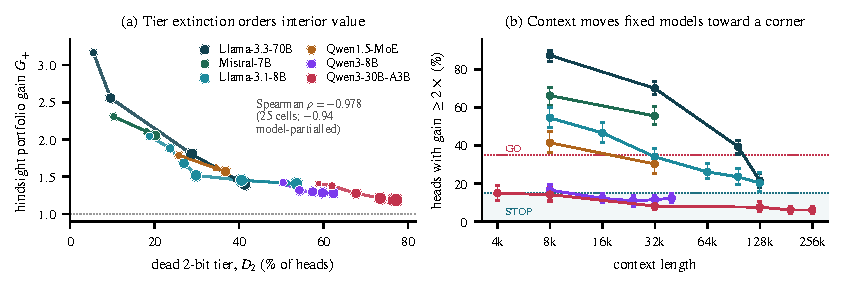
\includegraphics[width=\linewidth]{figures/fig1_regime.pdf}
  \vspace{-4mm}
  \caption{\textbf{F1--F2: where the interior lowers output error.} Mixed allocator and eviction endpoint both use lagged information; exact recomputation scores both. \textbf{(a)} The tier-extinction coordinate $D_2$ orders hindsight portfolio gain $\gplus$ across 25 cells; arrows show increasing context. \textbf{(b)} Context moves each fixed model across predeclared output-error bands. Error bars are 90\% layer-cluster intervals. Thresholds are not universal across architectures.}
  \label{fig:regime}
  \vspace{-3mm}
\end{figure}

\paragraph{F1: Tier extinction orders the interior's value, but the crossing is per architecture.}
On the 16-cell grid, the symmetric contract keeps roughly half of the advantage seen under an asymmetric one (current-query allocator vs.\ lagged eviction; Fig.~\ref{fig:evidence}a).  The symmetric band stays $1.2$--$12.5$ points above the all-oracle band in all 16 cells, five cells fall below 15\% (STOP), and $\gplus$ ranges from $1.05\times$ to $3.21\times$.  $D_2$ still orders the symmetric band ($\rho=-0.985$).  On the 25-cell extension, $D_2$ has Spearman $\rho=-0.978$ with both $\gplus$ and the band, and $-0.94$ with $\gplus$ ($-0.915$ with the band) after partialling out model identity (Fig.~\ref{fig:regime}a).  The crossing, however, is not universal.  Pooled monotone crossings sit near $D_2=29.0\%$ (GO) and $54.1\%$ (STOP) on the 25 cells, and at $26.8\%$ and $57.4\%$ on the 16-cell grid.  Yet Llama-3.1-8B keeps a $20.2\%$ band at $D_2=53.7\%$, while Qwen3-8B has $12.2\%$ at $D_2=54.3\%$: an eight-point gap across $0.6$ points of $D_2$, larger than prompt uncertainty.  $D_2$ is thus an ordering coordinate, and any operational boundary must be fitted per architecture.  The boundary also depends on the information contract.  On the same 16 cells, STOP is crossed at $D_2=46.9\%$ when both sides see the current query and at $57.4\%$ when both use lagged attention; this $10.5$-point shift exceeds either confidence interval.  Under the asymmetric contract STOP is never crossed.  $D_2$ itself is not sensitive in this way: two campaigns with different corner sets and code agree on it to within $0.30$ points in all 15 shared cells.

\paragraph{Why $D_2$ rather than a concentration or context statistic?}
We compared $D_2$ with simpler predictors on the same 25 cells, under a protocol fixed before computing them (Table~\ref{tab:app-predictors}): attention concentration $\tau$, the spread of log token sensitivity (a heterogeneity statistic of the kind RateQuant uses~\citep{zuo2026ratequant}), attention entropy, and context length alone.  Within a model, every statistic that moves with context orders $\gplus$ almost perfectly (mean $\rho=-0.99$); the difference lies across architectures.  Pooled over models, $D_2$ reaches $\rho=-0.978$, against $-0.72$ for $\tau$ and heterogeneity and $-0.48$ for context alone.  A log-linear fit on five models predicts the sixth to within a factor of $1.12$ for $D_2$, against $1.15$ ($\tau$, heterogeneity) and $1.24$ (context).  $D_2$ is therefore most useful for comparing architectures, and its held-out advantage over dispersion statistics is modest.

\paragraph{F2: Context moves a fixed model toward the eviction corner.}
Every measured trajectory moves toward more tier extinction as context grows (Fig.~\ref{fig:regime}b).  Llama-3.3-70B goes from GO at 8k to NARROW at 128k; Qwen3-8B goes from NARROW at 8k to STOP by 16k.  The main driver is absolute length: attention concentration $\tau$ rises smoothly and convexly in $\log L$, and a pre-registered curve of that shape explains most of the rise.  Only at exactly the trained RoPE limit does $\tau$ exceed that curve, by about $+0.21$ in Qwen3-8B and Qwen3-30B; there is no excess in Llama-3.1-8B, or at $0.75$ of the limit.  Both context and architecture matter; the data do not support a universal RoPE-triggered transition.  The surrogate is useful but not exact: the median ratio of predicted to recomputed gain lies in $[0.79,1.34]$ (a fit check, not a held-out prediction).

\begin{figure}[t]
  \centering
  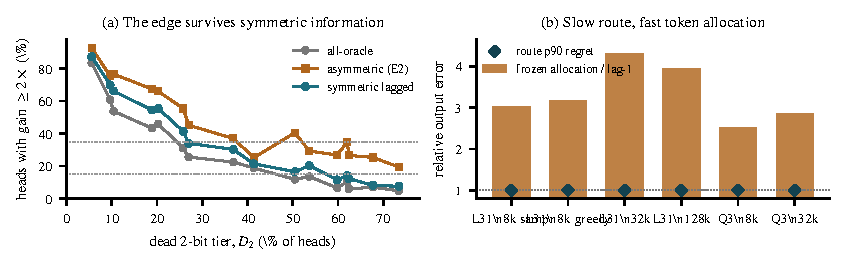
\includegraphics[width=\linewidth]{figures/fig2_evidence.pdf}
  \vspace{-4mm}
  \caption{\textbf{F1 robustness and F3 timescales.} \textbf{(a)} On the same 16 cells, the lagged-versus-lagged advantage is smaller than the asymmetric numbers (current-query interior against lagged eviction) but remains ordered by $D_2$. \textbf{(b)} In six cells, keeping the calibration-time \emph{policy family} has p90 regret $1.00$ through 4,096 generated tokens, whereas freezing the token assignment costs $2.52$--$4.30\times$ a one-step-old assignment.}
  \label{fig:evidence}
  \vspace{-3mm}
\end{figure}

\paragraph{F3: Two timescales, and the cost of acting on them.}
A head's output-error-optimal family (interior, uniform, or eviction) stays the same over 4,096 generated tokens in all six measured cells, but the token allocation inside a mixed head goes stale within a few steps (Fig.~\ref{fig:evidence}b).  A controller built on this map can therefore route rarely but must re-budget often.  Table~\ref{tab:deployment} (App.~\ref{app:robustness}) prices two constraints such a controller faces: sharing one allocation per GQA group costs $1.14\times$ at $n_{\rm rep}=4$, and the 4-bit cascade recovers 89\% of the staleness penalty.



% ===========================================================================
\section{Do output-distortion regimes transfer to end tasks?}
\label{sec:endtask}
% ===========================================================================

\begin{table}[t]
\centering
\footnotesize
\setlength{\tabcolsep}{2.6pt}
\caption{\textbf{End-task audit}: mean RULER score over valid cells (FP $=0.999$). \emph{Full grid}: 36 cells, one run each. \emph{8k}: all methods paired in one process (\S\ref{sec:protocol}).
Output error and effective bits ($B=2$) from the rerun. \emph{Hard}: Llama-3.1-8B, 32k, 32-key, $B=2$. Bold: best budget-matched; $^\ast$not matched (1 side bit/element). The router sends 1--25\% of KV heads to TurboQuant.
%\estalt{\est{Blue}: estimates awaiting runs (App.~\ref{app:ledger}).}{---: pending runs.}
}
\label{tab:endtask}
\begin{tabular}{@{}llrrrrrrrr@{}}
\toprule
& & \multicolumn{3}{c}{full grid (36 cells)} & \multicolumn{2}{c}{8k--32k rerun (28 cells)} & & & \\
\cmidrule(lr){3-5}\cmidrule(lr){6-7}
family & method & Llama & Qwen & all & Llama & Qwen & out.\ err. & eff.\ bits & hard \\
\midrule
\multirow{4}{*}{quant.} & TurboQuant-MSE & \textbf{0.985} & 0.867 & 0.946 & \textbf{0.995} & 0.874 & 0.445 & 2.12 & \est{0.88} \\
 & KIVI ($g{=}128$) & \est{0.96} & \est{0.98} & \est{0.97} & 0.965 & 0.986 & 0.298 & 2.25 & \est{0.85} \\
 & KIVI ($g{=}32$)$^\ast$ & \est{0.99} & \est{0.99} & \est{0.99} & 0.991 & 0.998 & 0.203 & 3.00 & \est{0.88} \\
 & KVQuant & \est{0.98} & \est{0.98} & \est{0.98} & 0.981 & \textbf{0.987} & 0.161 & 2.33 & \est{0.88} \\
\midrule
\multirow{6}{*}{eviction} & H2O & \est{0.36} & \est{0.34} & \est{0.35} & 0.355 & 0.340 & 0.345 & 2.04 & \est{0.25} \\
 & SnapKV & 0.479 & 0.237 & 0.398 & 0.385 & 0.222 & 0.290 & 2.04 & \est{0.21} \\
 & DropKV & 0.459 & 0.334 & 0.418 & 0.345 & 0.327 & 0.310 & 2.04 & \est{0.18} \\
 & Ada-KV & 0.612 & 0.285 & 0.503 & 0.550 & 0.259 & 0.289 & 2.04 & \est{0.25} \\
 & LaProx & 0.640 & 0.457 & 0.579 & 0.583 & 0.453 & 0.294 & 2.04 & \est{0.32} \\
 & OBCache-K + Ada-KV & 0.719 & 0.369 & 0.602 & 0.624 & 0.322 & 0.298 & 2.04 & \est{0.39} \\
\midrule
\multirow{2}{*}{mixed} & \sieve{} interior only & 0.479 & 0.438 & 0.465 & 0.458 & 0.463 & 0.150 & 2.07 & \est{0.28} \\
 & \sieve{} (router) & 0.654 & \textbf{0.989} & 0.766 & 0.692 & 0.962 & \textbf{0.135} & 2.08 & \est{0.32} \\
%\midrule
%\multirow{2}{*}{diag.} & \sieve{}, pooled score & --- & --- & --- & 0.756 & 0.581 & 0.177 & 2.07 & --- \\
% & \sieve{}, oracle router & --- & --- & --- & 0.815 & 0.981 & 0.121 & 2.08 & --- \\
\bottomrule
\end{tabular}
\vspace{-2mm}
\end{table}

%\tbd{[R12-A] 32k/128k paired rerun (replaces full-grid columns and Fig.~\ref{fig:endtask}). [R12-B] Hard cell; gate FP $\ge0.95$, TurboQuant in $[0.50,0.90]$ (at risk: 0.90/0.90 on calibration). [R12-D] Mistral evaluation.}

\paragraph{F4: Routed per head, the output-error optimum beats every eviction method, but a model-matched dense quantizer beats it.}
Table~\ref{tab:endtask} and Fig.~\ref{fig:endtask}a show three regularities.  First, routed per KV head, \sieve{} beats every eviction method.  Over the full grid it scores 0.766 against 0.602 for OBCache-K + Ada-KV ($+0.16$, 90\% CI $[+0.13,+0.20]$ by prompt bootstrap).  In the paired rerun it beats every eviction method on average, including H2O (0.808 vs.\ at most 0.527), with less than half their output error.  Part of this gain comes from routing 1--25\% of KV heads to dense (TurboQuant) quantization: the interior alone scores 0.465, below OBCache-K + Ada-KV, LaProx, and Ada-KV.  On Qwen3-8B, routing 9--18\% of heads to dense quantization lifts the score from 0.438 (interior) to 0.989, above TurboQuant alone (0.867).  Second, on Llama-3.1-8B, keeping every token at low precision wins.  TurboQuant scores 0.985, and at $B=2$ every eviction or mixed method trails it by at least $0.35$ (best: OBCache-K + Ada-KV, 0.626 vs.\ 0.976; \sieve{}, 0.429).  Third, on Qwen3-8B at $B=2$, TurboQuant's per-token rotated keys break down on variable tracking ($0.46$ at 8k, $0.40$ at 32k).  This reversal belongs to TurboQuant, not to dense quantization.  In the paired rerun the per-channel quantizers recover Qwen at both 8k and 32k: KIVI-128 scores 0.986 and KVQuant 0.987, above \sieve{} (0.962), with only 0.17--0.25 more effective bits.  KIVI-32 scores 0.998 but spends 3.00 effective bits against \sieve{}'s 2.08, so we do not treat it as budget-matched.  Mistral-7B follows Llama (10 valid cells, 8k and 32k): TurboQuant scores 0.951, KVQuant 0.861, and KIVI-128 0.825, against 0.699 for \sieve{} (interior alone: 0.070), which still leads every eviction method by a wide margin (best: 0.139).  So on all three models a budget-matched dense quantizer beats every eviction and mixed policy, as a broad benchmark found for quantization versus token dropping~\citep{yuan2024kvbench}, but which one depends on the model.  The pre-registered correlation between the output-error band and the router's accuracy gain is $-0.70$, opposite in sign to the prediction.  All 10 full-grid cells where \sieve{} trails the best eviction method by more than the run-to-run spread (0.15) are on Llama, 7 of them at 128k (Table~\ref{tab:app-h2h}).

\begin{figure}[t]
  \centering
  \ifshowest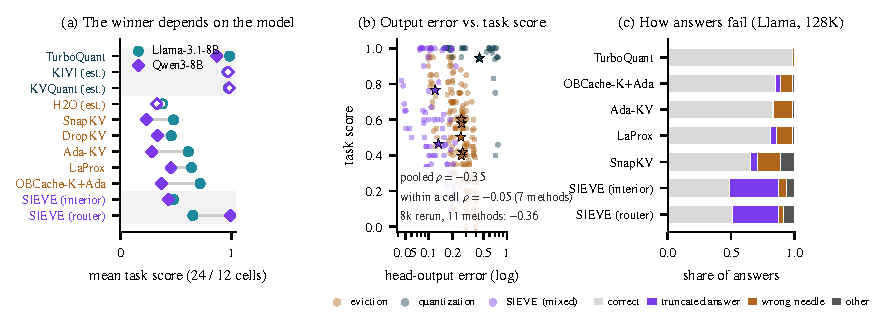
\includegraphics[width=\linewidth]{figures/fig3_endtask.pdf}\else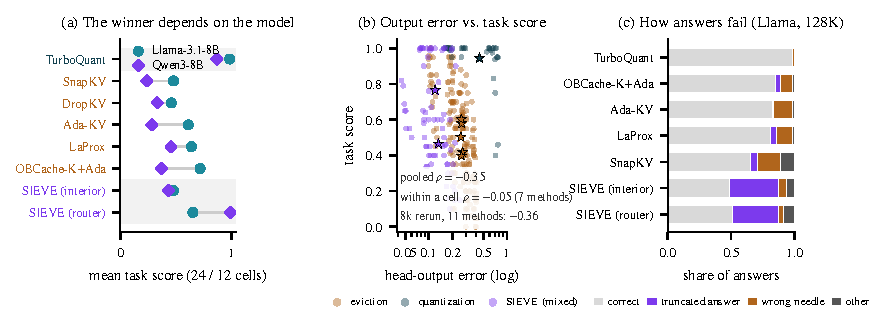
\includegraphics[width=\linewidth]{figures/fig3_endtask_noest.pdf}\fi
  \vspace{-4mm}
  \caption{\textbf{F4--F6: what transfers to task accuracy.} \textbf{(a)} Mean task score per method and model over the full grid; 
  %\estalt{hollow markers are estimates awaiting runs (App.~\ref{app:ledger}): KIVI, KVQuant and H2O, guided by the 8k rerun (Table~\ref{tab:endtask}).}{KIVI, KVQuant and H2O are so far measured only in the 8k rerun (Table~\ref{tab:endtask}).} 
  TurboQuant wins on Llama-3.1-8B; on Qwen3-8B \sieve{} beats TurboQuant but not the per-channel quantizers. \textbf{(b)} Head-output error vs.\ task score for every full-grid (cell, method); stars are method means. Error tracks accuracy across budgets and contexts; across methods it is weak, and TurboQuant (dark, top right) combines the highest error with the highest accuracy. \textbf{(c)} Single- and multi-key answers at Llama-3.1-8B, 128k, $B\in\{2,3\}$: \sieve{} fails by \emph{truncating} the correct number, eviction methods by returning a wrong needle.}
  \label{fig:endtask}
  \vspace{-3mm}
\end{figure}

\paragraph{F5: Output distortion ranks budgets and contexts well and methods weakly.}
\sieve{} minimizes the distortion it targets and has the lowest head-output error (0.120 on the full grid, 0.135 in the paired rerun), yet dense quantizers beat it.  Fig.~\ref{fig:endtask}b separates two uses of the proxy.  Across budgets and contexts, error and accuracy move together ($\rho=-0.69$ within the eviction family on the full grid).  Across methods at a fixed budget, the relation is weak and depends on which methods are compared.  The mean within-cell rank correlation is $-0.05$ over the eight full-grid methods and $-0.29$ over the twelve methods of the paired rerun ($-0.39$ among the eight eviction and mixed policies, $-0.10$ among the four dense quantizers); on Mistral-7B it is $-0.40$ (twelve methods).
TurboQuant is the clearest exception: its rotated, spread-out noise gives the highest output error (0.44) yet the highest Llama accuracy, whereas per-channel quantizers have both low error and high accuracy.
Output distortion therefore helps size budgets, but it overstates the cost of rotated quantization noise and should not be used to choose between families.
%\tbd{[R12-A] Recompute these correlations on the full paired grid.}
The router's calibration costs some accuracy but is not the main cause:
routing each head on its \emph{measured} test-prompt error raises the score only from 0.808 to 0.886 (Llama: 0.692 to 0.815). %, still below every dense quantizer.
The allocator is optimal for its own objective;
what fails is the transfer from that objective to retrieval.

\paragraph{F6: Token-granular allocation truncates multi-token answers; positional smoothing largely repairs it.}
\sieve{}'s weakest setting is Llama-3.1-8B at 128k, where it trails OBCache-K + Ada-KV by $0.32$ at $B=2$ (0.442 vs.\ 0.762).  Its wrong answers have a distinctive form (Fig.~\ref{fig:endtask}c).  Asked for 4929054, it answers ``492''; for 9465170, ``946''; for 6022964, ``602296''.  Llama tokenizes digits in groups of three, so the allocator keeps the key and the first token of the value but loses or garbles the rest.  We call an answer \emph{truncated} when it keeps the correct first three digits but is not the correct number.  Truncation accounts for 36\% of \sieve{}'s single- and multi-key answers at 128k (39\% for the interior alone; proper prefixes alone, 23\% and 28\%), against 1--11\% for every eviction method; those instead fail by returning a different needle (10--18\%).  Truncation is not specific to 128k: pooled over Llama's three contexts, 40\% of the interior's answers are truncated, although eviction methods also truncate 10--26\% at 8k and 32k, so the gap is widest at 128k.  The router does not rescue these heads, because by its objective the interior is the right choice.  At 128k it sends 99\% of Llama's KV heads to the interior, whose output error (0.094) is half that of any eviction method.  Losing the second token of one needle's value barely changes an error averaged over heads and decoding steps, but it changes the answer completely.

Why do the eviction methods avoid truncation?  Every one of them that beats \sieve{} here smooths its token scores over neighboring positions before selecting (max- or average-pooling over 7 positions).  A kept token thus protects its neighbors, and a needle survives as a phrase.  Pooling has its own cost: with several targets it can merge evidence that belongs to different ones~\citep{zhang2026fixedcontract}.  \sieve{}, in contrast, allocates each token independently from unpooled attention.  We pre-registered a test of this explanation: the same water-filling allocator on pooled attention supports it if it recovers at least half of the 128k, $B=2$ gap to OBCache-K + Ada-KV, and refutes it if it recovers less than one fifth.  The paired rerun already points in that direction.  On Llama-3.1-8B, pooling cuts truncated single- and multi-key answers from 39\% to 9\% at 8k and from 44\% to 11\% at 32k.  It raises the interior's mean score from 0.458 to 0.756, above OBCache-K + Ada-KV (0.624) and the calibrated router (0.692); at $B=2$ it moves the interior past OBCache at both contexts (8k: 0.299 to 0.663 vs.\ 0.446; 32k: 0.343 to 0.627 vs.\ 0.570).  Pooling helps less on Qwen3-8B (0.463 to 0.581; router 0.962).  On Mistral-7B the interior truncates as often as on Llama (39\%), but pooling cuts truncation only to 24\% (score 0.070 to 0.172); there the router, which sends 16\% of KV heads to dense quantization, does far better (0.699).  The pre-registered 128k cell remains the decisive test.
%\estonly{ (estimate \est{0.58}; half-gap threshold 0.59; oracle router \est{0.55})}.  
%\tbd{[R12-A, diagnostic arms] interior\_pool and router\_oracle at 128k.}

\paragraph{F7: Verdicts depend more on the comparison than on the sample.}
At both levels, the largest changes in a verdict came from what a method was compared against, and under which information contract, not from which prompts were drawn (Table~\ref{tab:contract}).  On the regime map, a new block of six prompts moves the band by a standard deviation of only $0.4$--$3.0$ points, so six prompts per cell suffice there.  Each of the other four choices in Table~\ref{tab:contract} moves a result by more than that and changes at least one verdict: the eviction corner, the information each side sees (F1), whether the question is visible when the cache is compressed, and which dense quantizer represents the endpoint (F4).
\begin{table}[t]
\centering
\small
\setlength{\tabcolsep}{4pt}
\caption{\textbf{F7:} how much each choice moves a verdict, compared with prompt sampling.}
\label{tab:contract}
\begin{tabular}{@{}p{0.34\linewidth}p{0.36\linewidth}p{0.22\linewidth}@{}}
\toprule
\textbf{Choice varied} & \textbf{Effect} & \textbf{Verdicts changed} \\
\midrule
Prompt block (sampling) & band s.d.\ $0.4$--$3.0$ pts, 4 cells & none \\
Eviction corner: accum vs.\ best of 5 & band $-5.1$ to $-8.6$ pts & 3 of 4 borderline cells \\
Information: current query vs.\ lagged & STOP crossing $46.9\%\to57.4\%$ $D_2$ & boundary location \\
Question visible at compression & SnapKV $0.11$--$0.65\to1.00$ in all 5 cells (same prompts); H2O changes by $\le0.08$ (8k, 32k) & every eviction ranking \\
Dense baseline: TurboQuant vs.\ per-channel & Qwen3-8B 8k--32k: $0.87\to0.99$ (KIVI-128, KVQuant) & \sieve{} vs.\ dense on Qwen \\
\bottomrule
\end{tabular}
\vspace{-2mm}
\end{table}


% ===========================================================================
\section{Implications}
\label{sec:implications}
% ===========================================================================

Five practical conclusions follow, each bounded by the retrieval tasks and models measured so far.
\begin{enumerate}[leftmargin=*,itemsep=1pt,topsep=2pt]
  \item \textbf{Report dense low-bit quantization, with more than one quantizer, next to any eviction or mixed method.}  On all three end-task models a dense quantizer beats every eviction and mixed policy we test at 2--3 key code bits, but not always the same one: TurboQuant on Llama-3.1-8B and Mistral-7B, per-channel KIVI and KVQuant on Qwen3-8B, where TurboQuant loses to \sieve{}.
  \item \textbf{Use output distortion to size budgets, not to choose methods.}  It orders settings well (F1, F5) and methods weakly, and overstates the cost of rotated quantization noise (F5).  Routing between method families needs a task-aware signal.
  \item \textbf{Allocate spans, not tokens.}  Token-separable objectives cannot see that a multi-token answer is only useful whole (F6).  Smoothing the allocator's scores over neighboring positions, which leaves Eq.~\ref{eq:discrete} intact, already cuts truncation from about 40\% to 10\% on Llama at 8k and 32k.
  \item \textbf{Name the comparison set and information contract with every verdict.}  They move results more than the prompt sample does (F7).
  \item \textbf{Calibrate per architecture and per context, and re-budget often.}  Crossings are architecture-specific and move with context (F1, F2); allocations go stale within steps (F3).
\end{enumerate}

%\paragraph{Scope of the budget comparison.}  Methods are compared at matched key code bits, with side information reported as effective bits (Table~\ref{tab:endtask}, App.~\ref{app:endtask}).  Quantization is simulated, so we make no memory-traffic or latency claims.

% ===========================================================================
\section{Related work}
\label{sec:related}
% ===========================================================================

\paragraph{Dense KV quantization.}
Dense quantizers store every token at low precision: per-channel or per-token integer schemes~\citep{liu2024kivi,hooper2024kvquant}, low-rank and sparse residual correction~\citep{kang2024gear}, rotations and sketches~\citep{zandieh2024qjl,zandieh2025turboquant}, and importance-aware mixed precision~\citep{yang2024mikv,he2024zipcache}.  RateQuant allocates finite precision across K/V heads from fitted distortion curves~\citep{zuo2026ratequant}.  Block-scaled 4-bit formats now make such caches native to hardware: the MX formats~\citep{ocp2023mx} and NVFP4, whose 16-element blocks carry FP8 scales~\citep{alvarez2025nvfp4}, including an NVFP4 KV cache~\citep{alvarez2025nvfp4kv}.
\paragraph{Eviction and sparse attention.}
Evictors keep recent and sink tokens~\citep{xiao2024streamingllm}, accumulate attention~\citep{zhang2023h2o,liu2023scissorhands}, use the last query~\citep{oren2024tova} or a prefill observation window~\citep{li2024snapkv}, and split budgets across layers and heads~\citep{cai2024pyramidkv,feng2024adakv}.  
Output-aware scores estimate the attention-output perturbation of removing a token: exactly for a singleton~\citep{goel2025caote}, under perturbation constraints~\citep{feng2026criticalkv}, by decoupled residual-output perturbation~\citep{zhang2026dropkv}, by Optimal-Brain-Damage saliency~\citep{gu2026obcache}, through the value and output projection with a model-wide budget~\citep{mai2026laprox}, or by layer-wise reconstruction with spatial-temporal smoothing~\citep{an2026restkv}. 
 Query-aware sparsity keeps the whole cache and selects pages per query~\citep{tang2024quest}, and reasoning-oriented methods target long generated traces~\citep{cai2025rkv,mao2026triattention}.  
%We evaluate six of these methods at matched key bits.  
Our truncation finding (F6) suggests one reason the strongest ones work: most smooth their scores over neighboring positions.  %which protects multi-token spans in a way a token-separable output-error objective does not.  
We claim not output-aware eviction but the separable approximation that puts zero rate inside a finite-rate allocator.

\paragraph{Hybrid storage and rate allocation.}
DiffKV routes tokens among high precision, low precision, and pruning with an on-GPU manager~\citep{zhang2025diffkv}, and HqeKV optimizes among full precision, several quantized levels, and eviction using joint K--V importance~\citep{wang-etal-2026-hqekv}.  
Concurrent work RDKV derives joint eviction--quantization rate allocation, assigning zero-to-finite rates to value tokens and key channels with packed decode~\citep{zhang2026rdkv}, and concurrent attention-aware transform coding applies output-aware reverse water-filling to transformed K/V channels~\citep{laus2026aatc}.  
Our allocation unit is the within-head key token, and our question is not whether water-filling can be derived but when its interior pays and whether the answer survives the step to task accuracy. 
Head, channel, and token axes are potentially composable (Table~\ref{tab:related}, App.~\ref{app:related}).

\paragraph{Diagnostics, evaluation contracts, and systems.}
A broad benchmark already found that KV quantization is reliable across task types while token dropping excels only on some, that compressing during prefill hurts retrieval, 
and that a model can emit a passkey's first digits before compression takes effect~\citep{yuan2024kvbench}.  
%Our dense-versus-eviction result agrees with the first finding.  %We add that the best quantizer depends on the model (F4), that the distortion-optimal allocator loses because its proxy misranks methods (F5), and that the first-digits effect becomes systematic truncation under token-level allocation (F6).
\citet{zhang2026fixedcontract} hold an eviction selector's contract fixed (attention tensor, observation window, budget, projection rule) and vary one stage at a time. %, attributing failures to a mismatch between prefill and decode queries, to output-unaware scoring, or to a projection that fragments evidence across the budget, on the same three model families we use.  
Their study covers eviction alone at 5--10\% retention and finds that output-aware scoring helps in most cells where it has room to.  
Ours adds dense and mixed-precision policies and finds that output error fails at a different point: 
choosing \emph{between} families at a fixed budget (F5).  
Our truncation failure (F6) is an instance of their projection stage, produced by a mixed-precision allocator rather than a selector, and F7 carries their fixed-contract principle one level up, to the baselines and information contract under which a verdict is stated.
%Systems constraints on deployed eviction are discussed in App.~\ref{app:related}.

% ===========================================================================
\section{Limitations and conclusion}
\label{sec:conclusion}
% ===========================================================================

%End-task results cover several models and  synthetic retrieval tasks, 
%and F4--F6 may not hold for reasoning, summarization, or long generation, where a truncated span may matter less or more.  
Compression is key-only with exact values, and budgets match key code bits rather than total KV bytes. % and all quantization is simulated, so no memory or throughput claim is made.  
The regime crossing is architecture-specific, and the diffuse (uniform) side of the map has less support than tier extinction.
%\estonly{  Several end-task entries are estimates pending the runs listed in Appendix~\ref{app:ledger}.}

Within that scope, mixed allocation is not uniformly useful.  Tier extinction orders when the interior lowers output error, context moves a model toward a corner, and allocations go stale faster than routes.
On end tasks, the output-error optimum, routed per head, beats every evictor we test, partly by keeping some heads dense.  As prior benchmarks found, a model-matched dense quantizer does better still, and output distortion cannot identify it.
Truncation points to the unit of allocation, which positional smoothing begins to repair.  Verdicts depend more on the comparison contract than on sampling.

\label{main:end}

% Statements below follow the ICLR 2027 template; none counts toward the page limit.
\subsection*{AI use statement}

In this work, we used generative AI tools (an AI coding and writing assistant) for the following tasks that the ICLR policy requires us to disclose.
\emph{Method implementation:} implementing and testing the KIVI and KVQuant-style baseline quantizers, the end-task result readers, the predictor comparison, and the figure and table scripts.
\emph{Experiment-design feedback:} proposing parts of the end-task campaign, namely the harder 32-key operating point, the question-visible control, the third end-task model, the pooled-score and oracle diagnostic arms, the predictor-comparison protocol, and several of their pre-registered decision rules, all of which the authors reviewed before any run.
\emph{Hypothesis proposal and results interpretation:} proposing the positional-pooling explanation of answer truncation (F6), the cross-cutting observation on comparison contracts (F7), and interpretations of the end-task results.
\emph{Qualitative data analysis:} classifying the models' wrong answers as truncated, wrong-needle, or other by rule, from generated text.
We also used AI assistance, as the policy recommends disclosing, for editing code and job scripts, drafting and restructuring the paper (including its title and section structure), literature search and summarization, bibliography entries, and figure creation.
%\estonly{  The estimated values marked in the paper and their stated bases were proposed with AI assistance.}
We have not used generative AI tools to generate, alter, or impute measured data: every reported measurement is computed by the experiment code from model runs.  
AI tools were not used in earlier phases of the project. The key problem this paper studies, the theoretical framework in Section~\ref{sec:framework}, and the regime-map experiments were not developed by AI. 
We have reviewed all AI-assisted work.  AI-written code was checked with unit tests, including a check of the RoPE inversion against a real model's cache, and with end-to-end runs before any GPU campaign; reported statistics were recomputed from the raw result files by the same readers that generate the tables; literature summaries were checked against the cited papers, and bibliography entries against arXiv or publisher pages.  We take responsibility for the final content of this work, including text, claims, or artifacts produced with the aid of generative AI.

\subsection*{Ethics statement}

This work measures compression of the key-value cache of publicly released language models on synthetic retrieval tasks built from public-domain books (PG-19).  It involves no human subjects, no personal or sensitive data, and no new model training.  The experiments used GPU time on a shared academic cluster (Appendix~\ref{app:compute}).  To guard research integrity, each experiment's decision rules were written before its results were read, and negative outcomes are reported alongside positive ones. %\estonly{; estimated values are distinguished from measurements throughout}.

\subsection*{Reproducibility statement}

Section~\ref{sec:framework} and Appendices~\ref{app:derivation}--\ref{app:allocation} give the allocation problem, its approximations, and the discrete optimizer.  Section~\ref{sec:protocol} and Appendix~\ref{app:protocol} specify models, context lengths, budgets, information contracts, and the response statistics; Appendix~\ref{app:endtask} specifies the end-task protocol, prompt blocks, validity filter, budget and side-information accounting, and every baseline with its deviations from the original paper.  The anonymized supplementary code contains the measurement and end-task runners, the baseline implementations with their unit tests, the pre-registered plans and decision rules for each experiment, the readers that produce every table and figure from result files, and the job scripts with the exact arguments used.  All models are public checkpoints, the corpus is public, and prompt indices and random seeds are fixed and recorded with each result.  Appendix~\ref{app:compute} lists the hardware, software versions, and per-job resources.

\bibliography{sieve,concurrent,related}
\bibliographystyle{iclr2027_conference}

\clearpage
\appendix
%\section{Appendix (planned)}
\tbd{A.1 Measurement integrity: the validity gates (real-corpus enforcement, needle retrieval, probe/chunking equivalence) and the defects they catch.
A.2 The $\tau/\ln2$ ladder identity as a consistency check; the 2-bit quantizer acts as a universal logit temperature ($\alpha=0.941$--$0.944$).
A.3 Findings and negative results: why $\tau$ and $n_{95}/L$ fail as regime variables; the refuted absolute-support eviction budget; H2 (2-bit score ranking, $\rho=0.52$--$0.77$) and the move to a 3-bit base layer; Gaussian-logit simulation as a qualitatively wrong regime map.
A.4 Per-model tables at every context.}


\tableofcontents
\vspace{1em}
\hrule
\vspace{1em}

\section{Introduction: The KV-Cache Compression Dilemma}
In autoregressive Transformer generation, storing key and value vectors across long context windows consumes substantial GPU high-bandwidth memory (HBM). Prior research has largely diverged into two competing paradigms:
\begin{enumerate}
    \item \textbf{Token Eviction (Sparsification):} Discarding tokens perceived to be uninformative (e.g., StreamingLLM, $\text{H}_2\text{O}$, SnapKV) while retaining retained tokens at full precision.
    \item \textbf{Uniform Quantization:} Lowering the numerical bit-width of all cached key and value vectors uniformly across the context (e.g., 3-bit or 4-bit uniform quantization).
\end{enumerate}
The theory presented here unifies these two disparate strategies under a single information-theoretic rate-distortion framework, proving that token eviction is not an ad-hoc heuristic, but rather the boundary case of zero-bit quantization.


\section{Output Distortion and the Equivalence Principle}

\subsection{Standard Attention Formulation}
For a query vector $q \in \mathbb{R}^d$, key vectors $\{k_i\}_{i=1}^L \subset \mathbb{R}^d$, and value vectors $\{v_i\}_{i=1}^L \subset \mathbb{R}^{d_v}$:
\begin{align}
    s_i &= \frac{q^\top k_i}{\sqrt{d}} \quad \text{(Pre-softmax logits)}, \\
    a_i &= \frac{\exp(s_i)}{\sum_j \exp(s_j)} = [\mathrm{softmax}(s)]_i \quad \text{(Attention weights)}, \\
    o &= \sum_{i=1}^L a_i v_i \quad \text{(Attention head output)}.
\end{align}

\subsection{Quantization Perturbation Model}
When key $k_i$ is quantized using $b_i$ bits, the resulting logit $s_i$ undergoes a perturbation $\delta_i$:
\begin{equation}
    \tilde{s}_i = s_i + \delta_i, \quad \mathrm{Var}(\delta_i) = \tau^2 c_{b_i},
\end{equation}
where:
\begin{itemize}
    \item $\tau$ denotes the \textbf{head logit spread} (the dynamic range or standard deviation of the logits for that specific attention head).
    \item $c_{b_i}$ is the \textbf{relative distortion factor} of the quantizer at bit-width $b_i$. For standard quantizers, distortion decays exponentially: $c_b \propto 4^{-b} = 2^{-2b}$.
    \item Any constant bias in the perturbation is completely neutralized because the softmax operator is shift-invariant: $\mathrm{softmax}(s + C \cdot \mathbf{1}) = \mathrm{softmax}(s)$. Thus, mean shift costs nothing, and only the variance $\mathrm{Var}(\delta_i)$ induces output error.
\end{itemize}

\subsection{First-Order Taylor Approximation of Output Error}
Differentiating the output vector $o$ with respect to logit $s_i$:
\begin{equation}
    \frac{\partial o}{\partial s_i} = \sum_{j} \frac{\partial a_j}{\partial s_i} v_j = a_i (v_i - o).
\end{equation}
Assuming independent perturbations across tokens, the expected squared distortion in the head output vector $o$ to first order is:
\begin{equation}
    \label{eq:distortion}
    \mathbb{E}\|\Delta o\|^2 \approx \sum_{i=1}^L a_i^2 \|v_i - o\|^2 \tau^2 c_{b_i}.
\end{equation}

\subsection{Eviction as Zero-Bit Quantization}
If a subset of tokens $E$ is evicted entirely and the remaining attention weights are renormalized, the leading-order output perturbation is:
\begin{equation}
    \|\Delta o_{\mathrm{evict}}\|^2 \approx \sum_{i \in E} a_i^2 \|v_i - o\|^2.
\end{equation}
Comparing this directly to Equation~\eqref{eq:distortion}, eviction precisely matches the quantization error formula when:
\begin{equation}
    \tau^2 c_0 = 1 \implies c_0 = \frac{1}{\tau^2}.
\end{equation}
\begin{remark}[\textbf{Fundamental Result}]
Eviction is identical to a quantizer rung at $b_i = 0$. Its cost constant $c_0$ is mathematically derived from the curvature of the softmax operator rather than being hand-tuned as an empirical penalty.
\end{remark}


\section{Optimal Rate Allocation via Reverse Water-Filling}

\subsection{The Constrained Optimization Problem}
Given a total bit budget of $BL$ bits across $L$ tokens (an average precision of $B$ bits per token), the objective is to choose $\{b_i\}_{i=1}^L$ to minimize output distortion:
\begin{equation}
    \min_{\{b_i\}} \sum_{i=1}^L a_i^2 \|v_i - o\|^2 \tau^2 c_{b_i} \quad \text{subject to} \quad \sum_{i=1}^L b_i \le B L, \quad b_i \ge 0.
\end{equation}

\subsection{Lagrangian Solution}
Using the distortion model $c_{b_i} \propto 4^{-b_i} = 2^{-2b_i}$, the Lagrangian separates independently for each token $i$. Setting the gradient with respect to $b_i$ to zero yields the water-filling solution:
\begin{equation}
    b_i^\star = \log_2 a_i + \log_2 \|v_i - o\| + c,
\end{equation}
where $c$ is a normalization constant determined by the total bit budget $BL$.
\begin{itemize}
    \item Tokens whose allocated bits exceed the threshold (above the ``water level'') are assigned $b_i^\star$.
    \item Tokens falling below the threshold are dropped to $b_i^\star = 0$ (\textbf{eviction}).
\end{itemize}

\subsection{The Value-Free Simplification}
Empirical measurements show that the variation of the value distance term $\log_2 \|v_i - o\|$ is negligible across tokens ($\le 0.035$ bits throughout real-world context data). Consequently, the value term can be absorbed into the constant:
\begin{equation}
    \label{eq:practical_wf}
    b_i^\star \approx \log_2 a_i + c.
\end{equation}
\textbf{Operational Significance:} Optimal bit allocation can be computed entirely from the attention weights $a_i$ alone, without requiring memory access to the value cache.


\section{Tier Extinction and the Order Parameter}

\subsection{The Convexity Condition}
On real hardware accelerators, bit-widths cannot vary continuously; they must belong to discrete rungs (e.g., $b \in \{0, 2, 4, 8\}$). A discrete tier $b$ is viable (lies on the lower convex envelope of the rate-distortion curve) if and only if storing a token at $b$ bits introduces less distortion than evicting it:
\begin{equation}
    \tau^2 c_b < \tau^2 c_0 = 1.
\end{equation}
\begin{definition}[\textbf{Dead Tier}]
If $\tau^2 c_b > 1$, tier $b$ is defined as \textbf{dead}. Storing a token at $b$ bits injects more variance into the logit than completely deleting the token. Therefore, no token should ever be quantized to $b$ bits.
\end{definition}

\subsection{The Two Asymptotic Regimes}
The inequality $\tau^2 c_b < 1$ determines the compression topology based on the head's logit spread $\tau$:
\begin{enumerate}
    \item \textbf{The Sharp End (High $\tau$, Large Dynamic Range):}
    As $\tau$ increases, $\tau^2 c_b$ exceeds 1 for low-bit precisions, killing rungs from the bottom up (e.g., 2-bit dies first, then 3-bit). Eventually, the available tier set collapses strictly to $\{0, b_{\max}\}$.
    $$\text{Optimal strategy} \longrightarrow \textbf{Pure Eviction (Keep at full precision or drop)}.$$
    
    \item \textbf{The Diffuse End (Low $\tau$, Small Dynamic Range):}
    When $\tau$ is small, the standard deviation of the log-attention weights collapses:
    \begin{equation}
        \mathrm{std}_i(\log_2 a_i) = \frac{\tau}{\ln 2} \to 0.
    \end{equation}
    The ladder spread shrinks below the width of a single rung, meaning all tokens receive essentially the same bit allocation.
    $$\text{Optimal strategy} \longrightarrow \textbf{Uniform Quantization}.$$
\end{enumerate}

\subsection{The Dead-Tier Fraction ($D_2$)}
To quantify model behavior, the \textbf{dead-tier fraction} $D_2$ is defined as:
\begin{equation}
    D_2 = \frac{1}{H} \sum_{h=1}^H \mathbb{I}\left(\tau_h^2 c_2 > 1\right),
\end{equation}
representing the proportion of attention heads where 2-bit quantization is inferior to eviction. $D_2$ acts as an order parameter: it requires only a single calibration pass, possesses zero free parameters, and is invariant to sequence length $L$.


\section{Empirical Evaluation Methodology}

\subsection{Experimental Architecture}
To test the analytical theory on real LLMs, an empirical testbed is structured as follows:
\begin{itemize}
    \item \textbf{Scale:} 24 distinct model/context configurations evaluated across 46,000 individual attention heads.
    \item \textbf{Context Scaling:} Context windows span every power-of-two from 8k tokens up to native model context limits.
    \item \textbf{Workload:} Synthetic ``needle-in-a-haystack'' retrieval embedded inside natural PG-19 book text.
    \item \textbf{Input-Validity Gate:} Strict verification ensuring that the uncompressed model successfully retrieves the needle on every prompt before testing compression.
\end{itemize}

\subsection{Quantization Engine and Scoring Integrity}
\begin{itemize}
    \item \textbf{Quantizer:} Key vectors are quantized using $\mathrm{TurboQuant}_{\mathrm{mse}}$, which combines random orthogonal rotations with Lloyd--Max optimal scalar quantization.
    \item \textbf{Strict Separation:} Equation~\eqref{eq:distortion} and Equation~\eqref{eq:practical_wf} are utilized \emph{exclusively} to plan bit assignments ($b_i^\star$). The recorded error is always the \textbf{exact recomputed output} $o$ evaluated through the real quantized key vectors.
\end{itemize}

\subsection{Matched-Budget Comparative Baselines ($B = 3$ bits/token)}
All techniques operate under an identical bit budget ($B = 3$ bits per token):
\begin{table}[h]
\centering
\small
\begin{tabular}{@{}lll@{}}
\toprule
\textbf{Compression Scheme} & \textbf{Mechanism} & \textbf{Regime Alignment} \\
\midrule
\textbf{Uniform Quantization} & Every token stored at exactly $b_i = 3$ bits & Diffuse Corner \\
\textbf{Pure Eviction} & Keep top $BL/8 = 3L/8$ tokens at 8 bits; evict the rest & Sharp Corner \\
\textbf{Water-Filling} & Allocates $b_i^\star \approx \log_2 a_i + c$ across discrete tiers & Intermediate Spectrum \\
\bottomrule
\end{tabular}
\caption{Matched-budget comparison at 3 bits/token. Eviction ranks tokens via $\text{H}_2\text{O}$ accumulated attention.}
\label{tab:baselines}
\end{table}

\subsection{Evaluation Metrics}
\begin{itemize}
    \item \textbf{Per-Head Gain:} The ratio of the best corner baseline error to the water-filling error:
    \begin{equation}
        \mathrm{Gain} = \frac{\min\left(\mathrm{Error}_{\mathrm{uniform}}, \, \mathrm{Error}_{\mathrm{eviction}}\right)}{\mathrm{Error}_{\mathrm{water\text{-}filling}}}.
    \end{equation}
    \item \textbf{In-Band Heads:} Attention heads exhibiting $\mathrm{Gain} \ge 2\times$, where mixed-precision water-filling outperforms both classical extremes by at least a factor of two.
    \item \textbf{Routed Gain:} The geometric mean of $\max(\mathrm{Gain}, 1)$, reflecting the real-world performance attained by a dynamic per-head router selecting the optimal compression scheme.
    \item \textbf{Symmetric Information Principle:} Allocation and corner baselines score token importance using identical attention statistics, ensuring fair benchmarking.
\end{itemize}


\section{Summary of Key Takeaways}
\begin{table}[h]
\centering
\small
\begin{tabular}{@{}p{0.28\textwidth}p{0.67\textwidth}@{}}
\toprule
\textbf{Core Concept} & \textbf{Key Takeaway} \\
\midrule
\textbf{Eviction is 0-bit quantization} & Setting $\tau^2 c_0 = 1$ naturally aligns token dropping with quantization theory; no separate eviction heuristic is needed. \\
\addlinespace
\textbf{Logit spread $\tau$ dictates policy} & High $\tau$ (sharp heads) kills low-bit tiers and favors pure eviction; low $\tau$ (diffuse heads) favors uniform quantization. \\
\addlinespace
\textbf{Value-cache independence} & Bit allocation depends almost entirely on $\log_2 a_i$, enabling optimal allocation without accessing or loading value vectors. \\
\addlinespace
\textbf{Hardware routing potential} & Modeling in-band heads enables per-head routing, optimizing accuracy per byte across heterogeneous attention layers. \\
\bottomrule
\end{tabular}
\caption{Summary of foundational insights.}
\label{tab:takeaways}
\end{table}





\end{document}
